\documentclass[12pt]{article}
\usepackage[spanish]{babel}
\usepackage{url}
\usepackage[utf8x]{inputenc}
\usepackage{blindtext}
\usepackage{amsmath}
\usepackage{graphicx}
\usepackage{float}
\usepackage{pdfpages}
\graphicspath{{images/}}
\usepackage{parskip}
\usepackage{fancyhdr}
\usepackage{vmargin}
\setmarginsrb{3 cm}{2.5 cm}{3 cm}{2.5 cm}{1 cm}{1.5 cm}{1 cm}{1.5 cm}

\title{Decide Ortosia - Autenticación}								%Title
								% Author
\date{12 Sept 2015}											% Date

\makeatletter
\let\thetitle\@title
\let\theauthor\@author
\let\thedate\@date
\makeatother

\pagestyle{fancy}
\fancyhf{}
\rhead{\theauthor}
\lhead{\thetitle}
\cfoot{\thepage}

\begin{document}

%%%%%%%%%%%%%%%%%%%%%%%%%%%%%%%%%%%%%%%%%%%%%%%%%%%%%%%%%%%%%%%%%%%%%%%%%%%%%%%%%%%%%%%%%

\begin{titlepage}
	\centering
    \vspace*{0.5 cm}
    
\includegraphics[scale = 0.2]{logo.png}\\[1.0 cm]	% University Logo
    \textsc{\LARGE Escuela Técnica Superior de Ingeniería  \newline\newline Informática}\\[2.0 cm]	% University Name
	\textsc{\Large Opera Id:125}\\[0.5 cm]				% Course Code
	\rule{\linewidth}{0.2 mm} \\[0.4 cm]
	{ \huge \bfseries \thetitle}\\
	\rule{\linewidth}{0.2 mm} \\[1.5 cm]
	
	\begin{minipage}{0.4\textwidth}
		\begin{flushleft} \large
			\emph{Autores:}\\
			González Jiménez, Álvaro \\		
			Rojas Gutiérrez, Rodrigo\\
            Romero Cáceres, Antonio\\
            Bonacini, Luca\\
            Millán García, Antonio \\
			\end{flushleft}
			\end{minipage}~
			\begin{minipage}{0.4\textwidth}
            
			\begin{flushright} \large
			\emph{Tutores:} \\
			David Benavides Cuevas\\
            \emph{Opera Id: }
            125\\
			\emph{Grupo: }            
            G1\\
            
            
		\end{flushright}
        
	\end{minipage}\\[2 cm]
	
	
    
    
    
    
	
\end{titlepage}

%%%%%%%%%%%%%%%%%%%%%%%%%%%%%%%%%%%%%%%%%%%%%%%%%%%%%%%%%%%%%%%%%%%%%%%%%%%%%%%%%%%%%%%%%

\tableofcontents
\listoftables
\pagebreak

%%%%%%%%%%%%%%%%%%%%%%%%%%%%%%%%%%%%%%%%%%%%%%%%%%%%%%%%%%%%%%%%%%%%%%%%%%%%%%%%%%%%%%%%%

\section{Diario de grupo}

\subsection{Hojas de tiempo}
\setboolean{@twoside}{false}
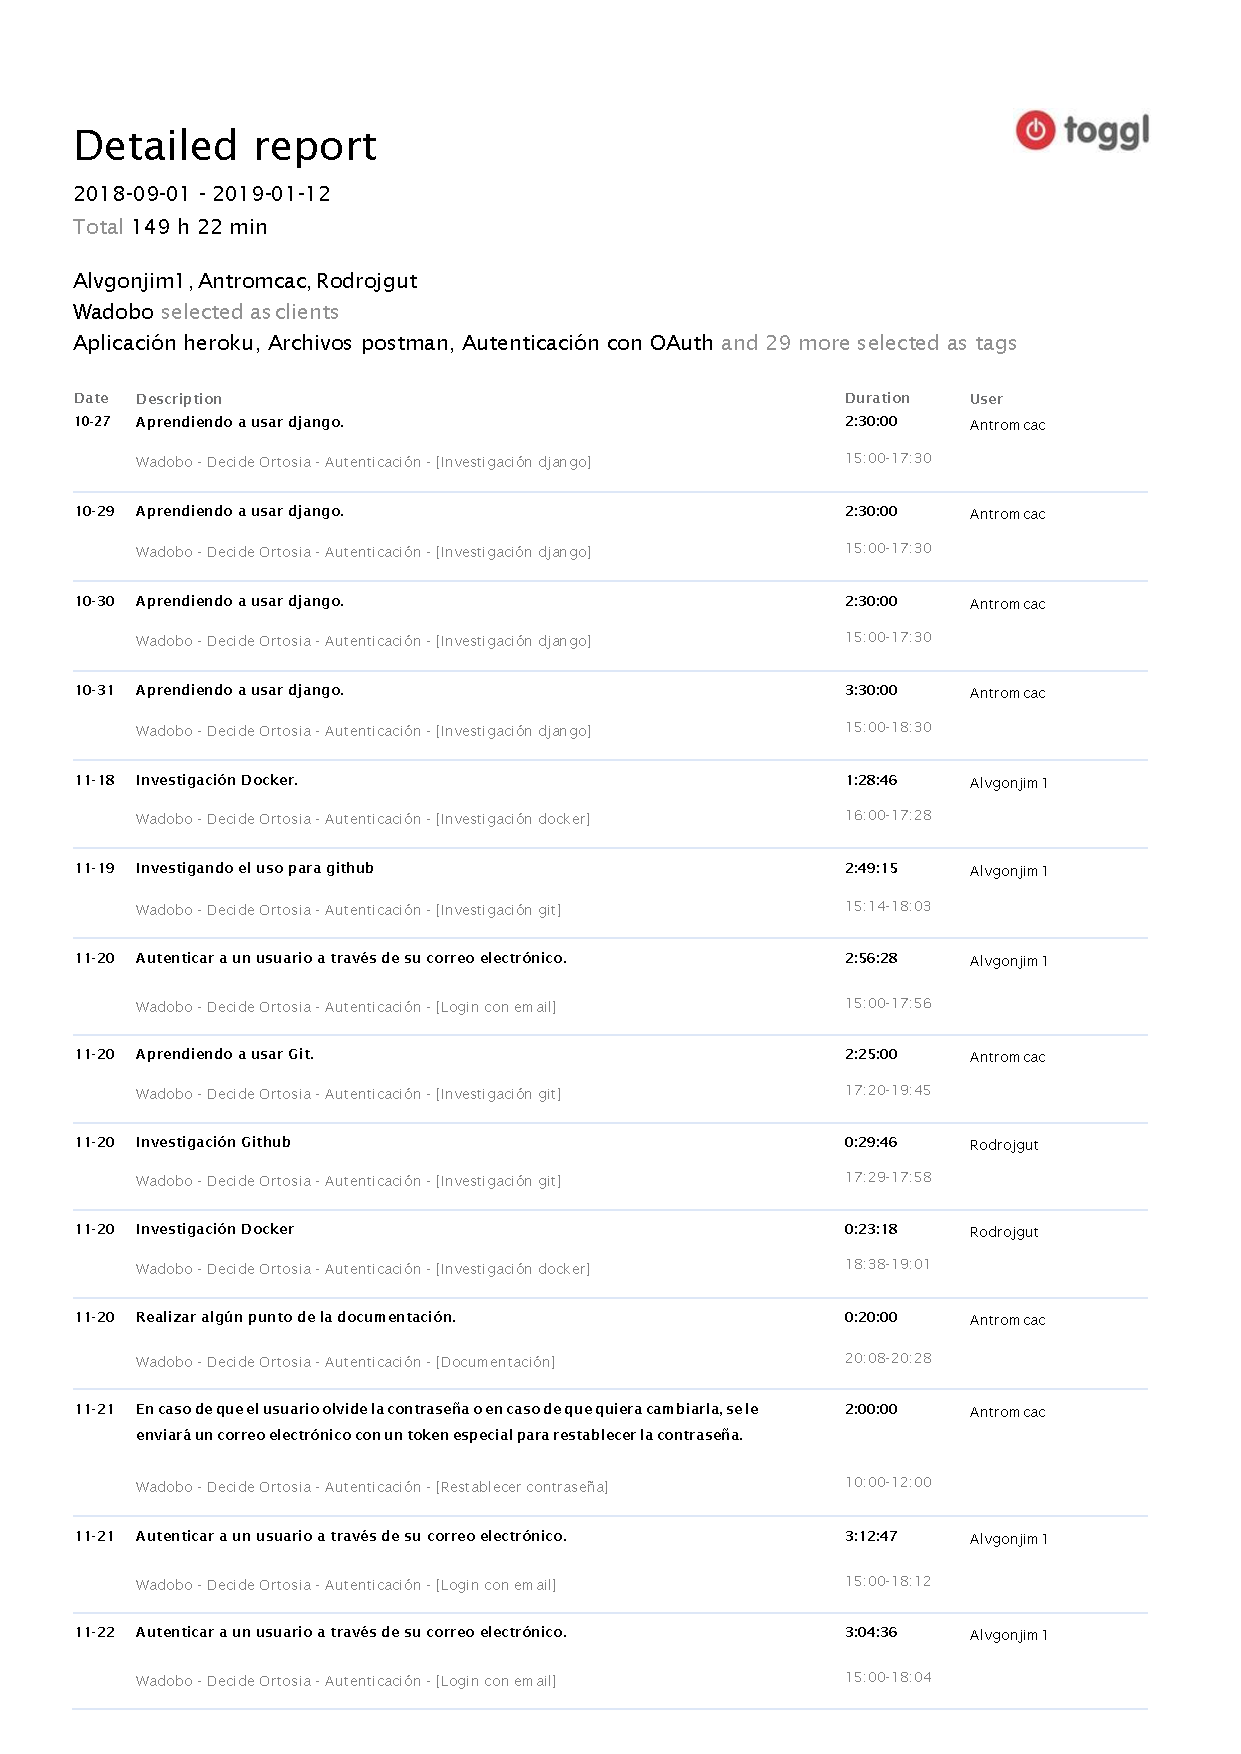
\includepdf[pages=-, offset=70 -70]{hojaDeTiempo.pdf}

\subsection{Reuniones}

\begin{table}[H]
\centering
\begin{tabular}{|c|c|c|}
\hline
\textbf{Fecha} & \textbf{Asistentes} & \textbf{Duración(horas)} \\ \hline
20/11/2018 & \begin{tabular}[c]{@{}c@{}}González Jiménez, Álvaro\\Rojas Gutiérrez, Rodrigo\\ Romero Cáceres, Antonio\end{tabular} & 1:00 \\ \hline
4/12/2018 & \begin{tabular}[c]{@{}c@{}}González Jiménez, Álvaro\\ Rojas Gutiérrez, Rodrigo\\ Romero Cáceres, Antonio\end{tabular} & 1:20 \\ \hline
02/01/2019 & \begin{tabular}[c]{@{}c@{}}González Jiménez, Álvaro\\ Rojas Gutiérrez, Rodrigo\\ Romero Cáceres, Antonio\end{tabular} & 0:45 \\ \hline
\end{tabular}
\caption{Reuniones}
\end{table}

\subsection{Duración total}

\begin{table}[H]
\centering
\begin{tabular}{|c|c|}
\hline
\textbf{Integrantes del grupo} & \textbf{Horas totales} \\ \hline
Álvaro González Jiménez & 60:55:58 \\ \hline
Rodrigo Rojas Gutiérrez & 44:11:54 \\ \hline
Antonio Romero Cáceres & 44:15:00 \\ \hline
\end{tabular}
\caption{Duración total}
\end{table}

\subsection{Dedicación}
\begin{table}[H]
\centering
\begin{tabular}{|c|c|c|}
\hline
\textbf{Alumno} & \textbf{Dedicación} & \textbf{Foto del alumno} \\ \hline
González Jiménez, Álvaro & 5 & {
\includegraphics[width=2cm, height=2cm]{./alvaro}} \\ \hline
Rojas Gutiérrez, Rodrigo & 5 & {
\includegraphics[width=20mm]{./rodrigo}} \\ \hline
Romero Cáceres, Antonio & 5 &  {
\includegraphics[width=20mm]{./antonio}}\\ \hline
Bonacini, Luca & 0 & \\ \hline
Millán García, Antonio & 0 &  \\ \hline
\end{tabular}
\caption{Dedicación}
\end{table}

\subsection{Actas de reuniones}
 Se encuentran anexadas al final del documento.
\section{anexos}
\setboolean{@twoside}{false}
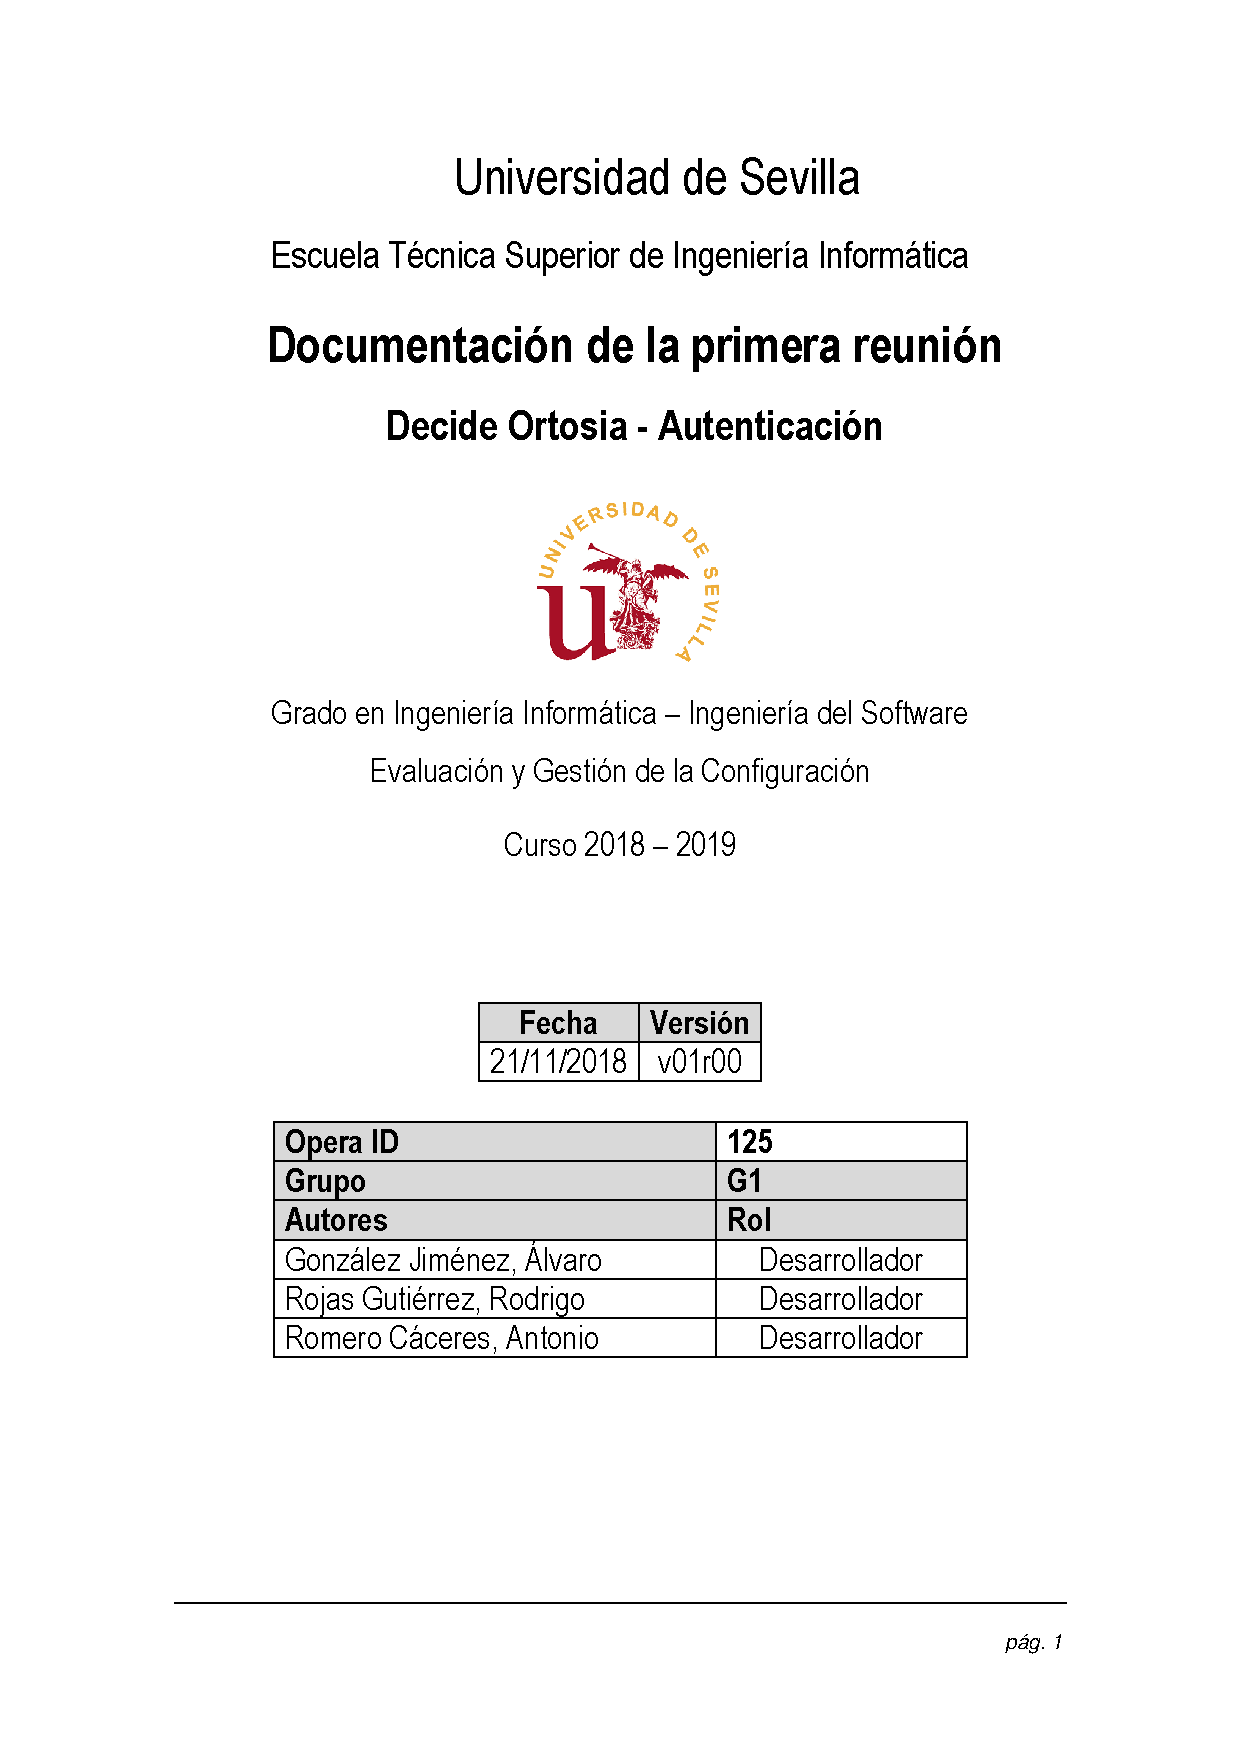
\includepdf[pages=-, offset=70 -70]{reunion1.pdf}
\setboolean{@twoside}{false}
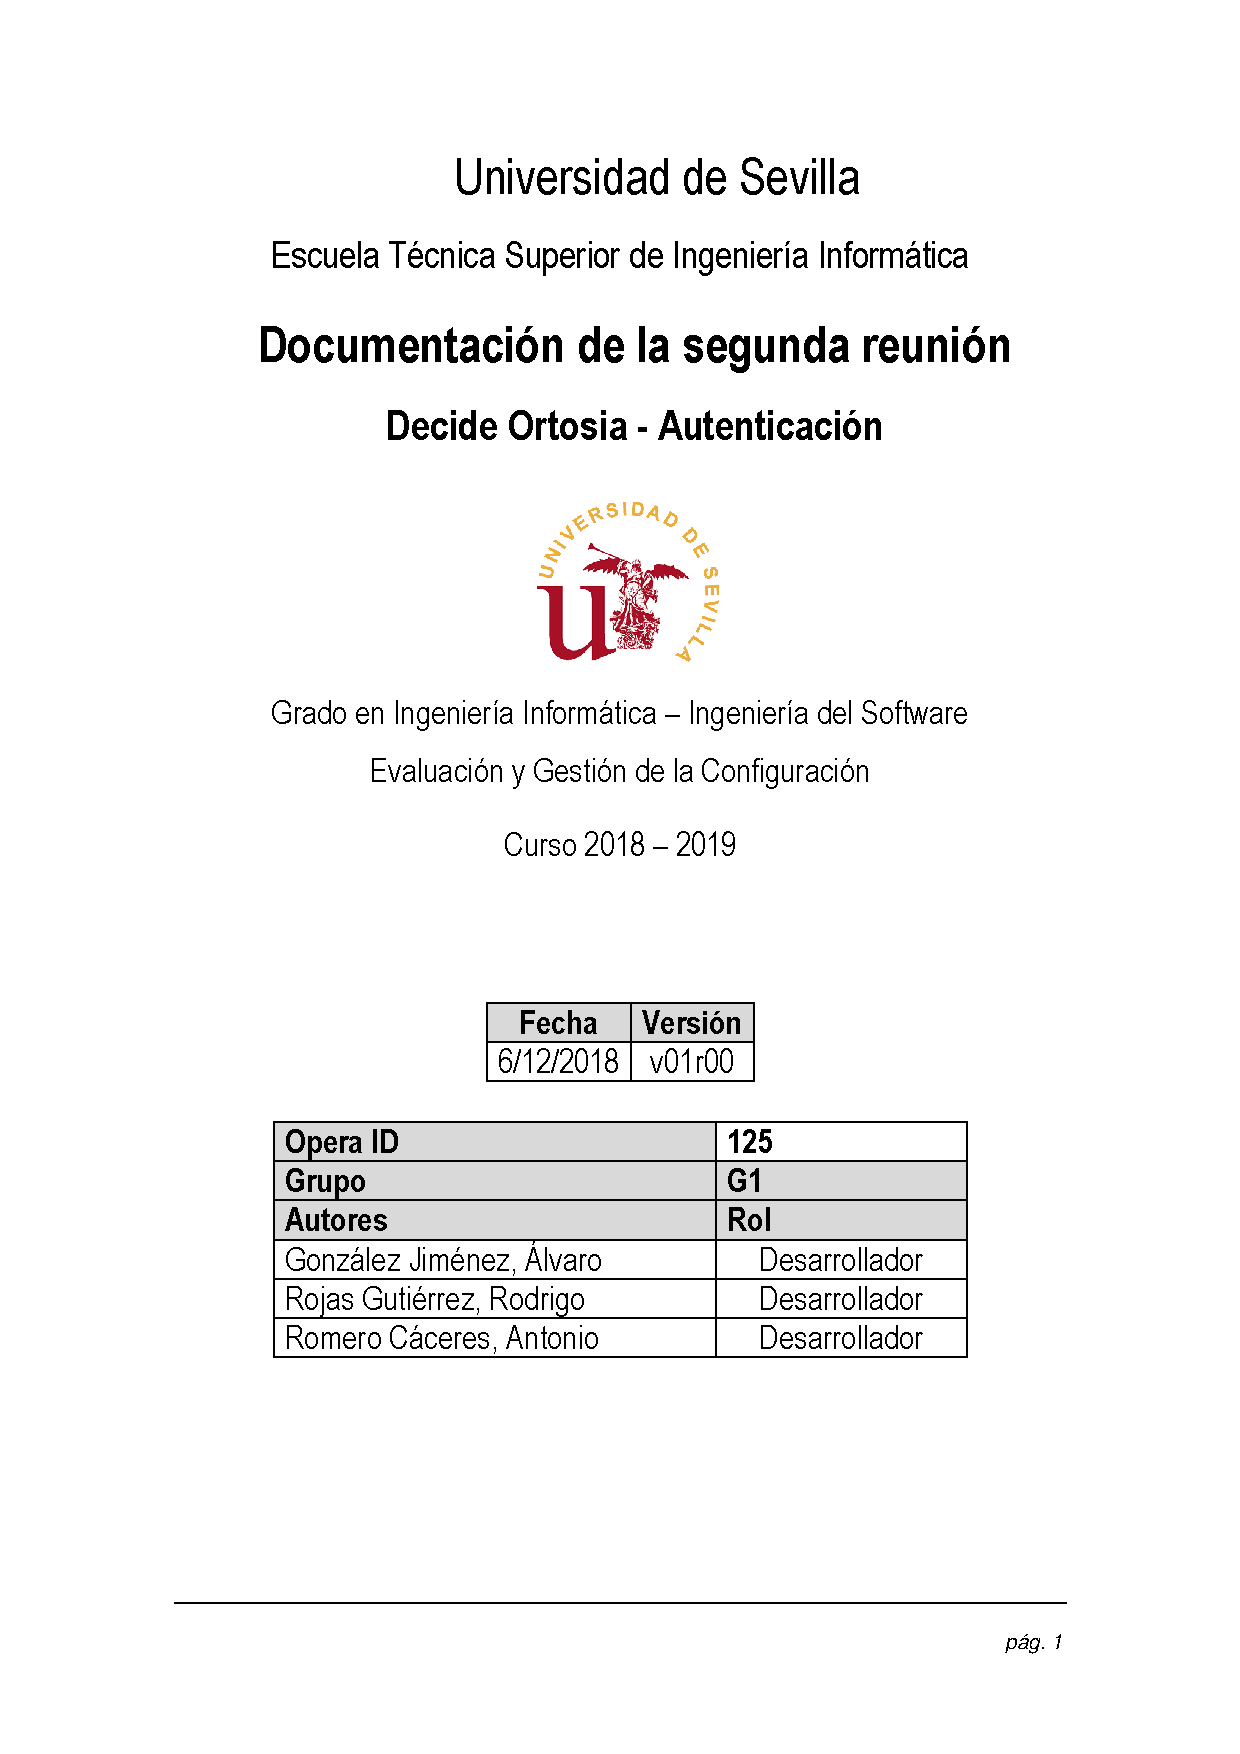
\includepdf[pages=-, offset=70 -70]{reunion2.pdf}
\setboolean{@twoside}{false}
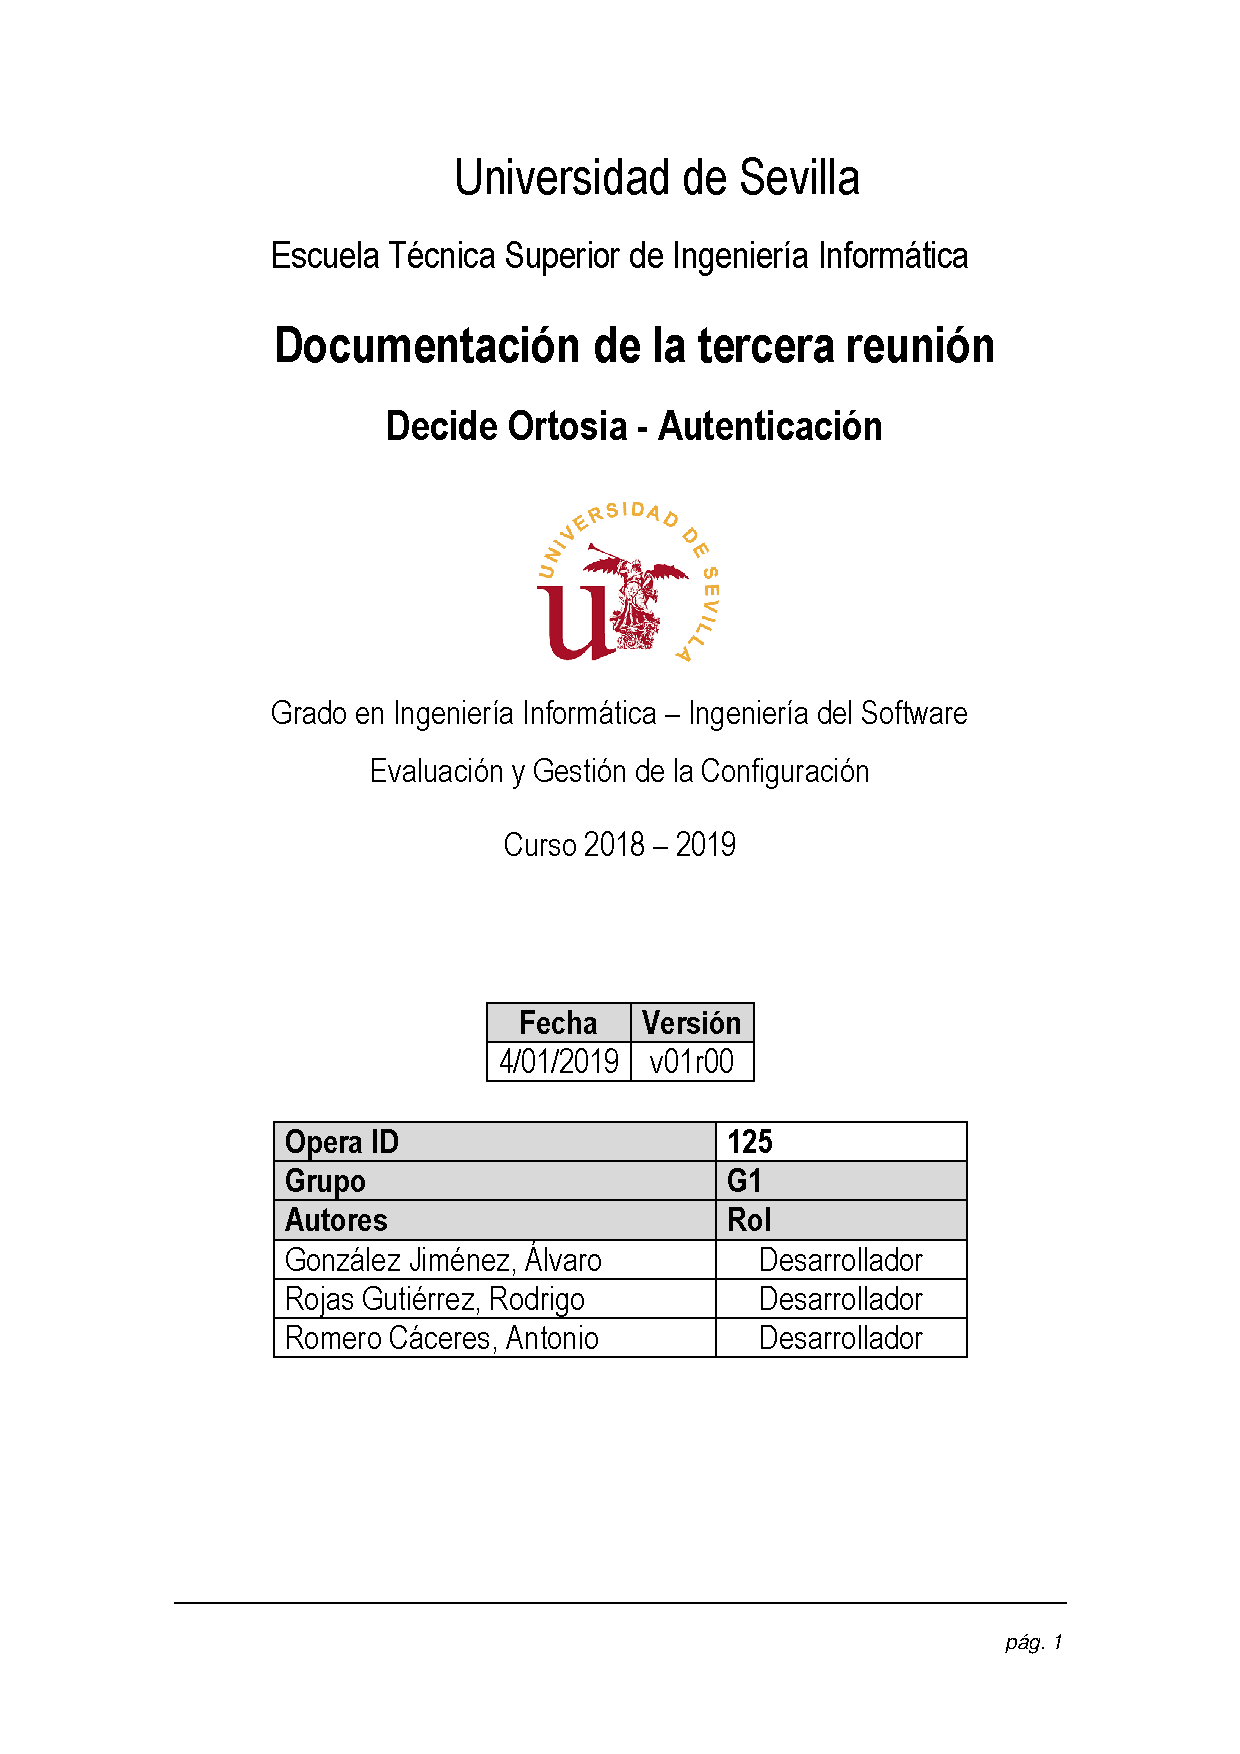
\includepdf[pages=-, offset=70 -70]{reunion3.pdf}
\end{document}